\documentclass[9pt]{extarticle}

\usepackage[T1]{fontenc}
\usepackage{lmodern}
\usepackage[letterpaper,left=0.5in,right=0.5in,top=0.5in,bottom=0.55in]{geometry}
\usepackage{microtype}
\usepackage{xcolor}
\usepackage{booktabs}
\usepackage{array}
\usepackage{xltabular}
\usepackage{enumitem}
\usepackage{tikz}
\usetikzlibrary{arrows.meta,positioning,calc}
\usepackage{caption}
\usepackage{float}
\usepackage{titlesec}
\usepackage[hidelinks]{hyperref}
\titlespacing*{\section}{0pt}{0.7em}{0.25em}
\titlespacing*{\subsection}{0pt}{0.45em}{0.1em}
\titleformat*{\subsection}{\normalsize\bfseries}

\setlist{nosep,leftmargin=1.4em}
\setlength{\parskip}{0.28em}
\setlength{\parindent}{0pt}
\setlength{\emergencystretch}{2em}
\renewcommand{\arraystretch}{1.04}
\captionsetup{font=small,labelfont=bf}

% Inline code: prints underscores and other symbols literally.
\newcommand{\code}[1]{\texttt{\detokenize{#1}}}
\newcolumntype{L}{>{\raggedright\arraybackslash}X}
\newcolumntype{P}[1]{>{\raggedright\arraybackslash}p{#1}}


\begin{document}
\begin{center}
{\LARGE\bfseries SilverFile: System Design Report}\\[4pt]
ENMGT 5405, Assignment 7 \,\textperiodcentered\, October 30, 2026 \,\textperiodcentered\, \url{https://github.com/tomas-schmieder/5405-Silverfile} \\[2pt]
{\small Hussain Al Shabib \quad Kezia Mally Puteri \quad Taylor Do \quad Anastasia Patrikiadou \quad Anjana \quad Tom\'as Schmieder}
\end{center}

%--------------------------------------------------------------------
\section{Overview and design goals}

SilverFile is a LangGraph multi-agent system that turns an intake conversation and uploaded tax documents into a \textbf{draft} 2025 Form 1040-SR, with a provenance record behind every dollar amount and a human reviewer for anything it should not decide. It has a deterministic orchestrator, six functional agents and one human-review node, and it runs with or without an Anthropic API key.

Five business rules from the brief shaped every design choice. Each is enforced in code, not only in prompts:

\begin{xltabular}{\linewidth}{@{}P{4.2cm}L@{}}
\toprule
\textbf{Rule} & \textbf{How the design enforces it} \\
\midrule
Never file anything & The only output is a filled PDF marked as a draft plus a JSON audit record. ``Submitted'' means submitted to a Kushim employee for review. \\
Never give tax advice & Intake detects advice, planning and optimisation requests and raises an \code{advice_request} escalation. The reviewer can only note the question or refer it. \\
Never assert an unsourced amount & Computation copies every number from a deterministic MCP tool result. Return Assembly refuses to produce a draft if any money line has a gap in its provenance chain. \\
Always route to a human when required & Every \S4.4 condition maps to a reason code that triggers a LangGraph \code{interrupt}. \\
Handle only the in-scope profile & Eligibility \& Rules screens for out-of-scope items during intake and again before computation; hard stops can only be referred out. \\
\bottomrule
\end{xltabular}

\textbf{Technology.} Python 3.12, LangGraph with a SQLite checkpointer, a stdio MCP server for all tax arithmetic, Streamlit for the taxpayer view and the employee dashboard, and \code{pypdf} to fill the official IRS 1040-SR and Schedule 1-A PDFs. In live mode, Claude reads documents and interprets free-text answers through structured outputs. In offline mode, a rule-based parser and bundled RapidOCR do the same, so graders can run every evaluation without a key or a network connection.

\textbf{Topology: hub and spoke around a rule-based orchestrator.} We chose this over a supervisor LLM or a peer-to-peer swarm for three reasons. Every hop is explainable from state and logged with a reason. Termination is guaranteed, because routing is code with an explicit priority order. And the business constraint that no agent may do another's job is easier to verify when all control transfer passes through one place. The trade-off is that new behaviour needs a code change to \code{decide()}, not a prompt change; for a regulated workflow we considered that a benefit.

%--------------------------------------------------------------------
\section{Orchestration}

Every agent returns control to the orchestrator, which picks the next node from the current state; there are no fixed agent-to-agent edges except the extraction fan-in.

\begin{figure}[H]
\centering
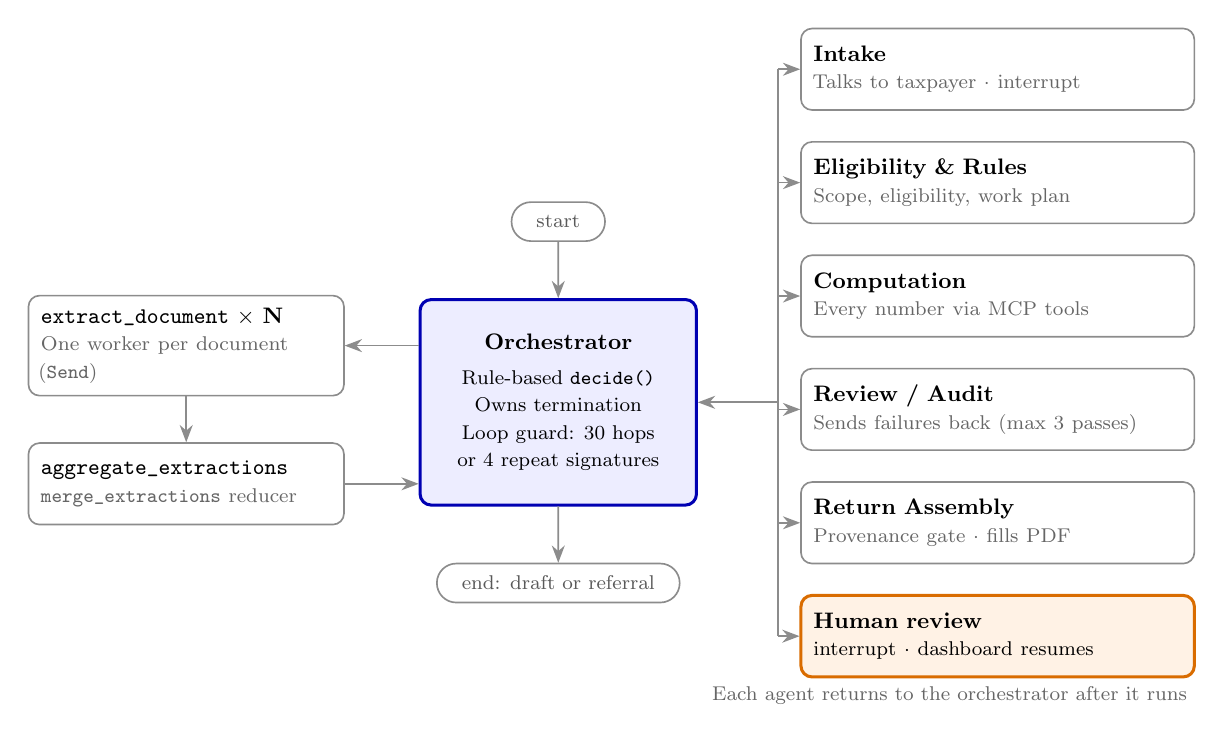
\begin{tikzpicture}[scale=0.9, transform shape,
    font=\small,
    >={Stealth[length=2.2mm]},
    line/.style={draw=black!45, line width=0.6pt},
    agent/.style={draw=black!45, line width=0.6pt, rounded corners=4pt,
                  minimum height=1.15cm, text width=5.2cm, align=left, inner sep=5pt},
    pill/.style={draw=black!45, line width=0.6pt, rounded corners=7pt,
                 minimum height=0.55cm, inner xsep=10pt, text=black!65, font=\footnotesize},
  ]
  % Orchestrator (hub)
  \node[draw=blue!70!black, fill=blue!7, line width=1.1pt, rounded corners=4pt,
        minimum width=3.9cm, minimum height=2.9cm, align=center] (orch) at (7.9,-6.3)
    {\textbf{Orchestrator}\\[3pt]
     \footnotesize Rule-based \code{decide()}\\
     \footnotesize Owns termination\\
     \footnotesize Loop guard: 30 hops\\
     \footnotesize or 4 repeat signatures};
  \node[pill] (start) at (7.9,-3.75) {start};
  \node[pill] (end) at (7.9,-8.85) {end: draft or referral};

  % Parallel extraction
  \node[agent, text width=4.1cm] (extract) at (2.65,-5.5)
    {\textbf{\code{extract_document} $\times$ N}\\
     {\footnotesize\color{black!60} One worker per document (\code{Send})}};
  \node[agent, text width=4.1cm] (agg) at (2.65,-7.45)
    {\textbf{\code{aggregate_extractions}}\\
     {\footnotesize\color{black!60} \code{merge_extractions} reducer}};

  % Functional agents (spokes)
  \node[agent] (intake) at (14.1,-1.6)
    {\textbf{Intake}\\{\footnotesize\color{black!60} Talks to taxpayer $\cdot$ interrupt}};
  \node[agent] (rules) at (14.1,-3.2)
    {\textbf{Eligibility \& Rules}\\{\footnotesize\color{black!60} Scope, eligibility, work plan}};
  \node[agent] (comp) at (14.1,-4.8)
    {\textbf{Computation}\\{\footnotesize\color{black!60} Every number via MCP tools}};
  \node[agent] (review) at (14.1,-6.4)
    {\textbf{Review / Audit}\\{\footnotesize\color{black!60} Sends failures back (max 3 passes)}};
  \node[agent] (asm) at (14.1,-8.0)
    {\textbf{Return Assembly}\\{\footnotesize\color{black!60} Provenance gate $\cdot$ fills PDF}};
  \node[agent, draw=orange!85!black, fill=orange!10, line width=1.1pt] (hr) at (14.1,-9.6)
    {\textbf{Human review}\\{\footnotesize interrupt $\cdot$ dashboard resumes}};

  % Connectors
  \draw[line,->] (start) -- (orch);
  \draw[line,->] (orch) -- (end);
  \draw[line,->] (orch.west |- extract.east) -- (extract.east);
  \draw[line,->] (extract) -- (agg);
  \draw[line,->] (agg.east) -- (orch.west |- agg.east);

  \coordinate (bus) at (11.0,-6.3);
  \draw[line,<-] (orch.east |- bus) -- (bus);
  \draw[line] (11.0,-1.6) -- (11.0,-9.6);
  \foreach \n in {intake,rules,comp,review,asm,hr}
    \draw[line,->] (11.0,0 |- \n.west) -- (\n.west);

  \node[anchor=north east, font=\footnotesize, text=black!60] at (hr.south east)
    {Each agent returns to the orchestrator after it runs};
\end{tikzpicture}
\caption{SilverFile orchestration graph (\code{src/graph.py}): hub and spoke, one parallel fan-out, one interrupt node.}
\label{fig:graph}
\end{figure}

The orchestrator is the only node with outgoing conditional edges. Extraction is the one parallel branch, and human review is the one place the graph pauses for a Kushim employee (Intake pauses separately for the taxpayer).

\textbf{Conditional routing.} \code{decide()} in \code{src/agents/orchestrator.py} evaluates a fixed priority list on each pass: (1)~terminal status ends the run; (2)~a pending escalation goes to \code{human_review}; (3)~queued documents fan out to \code{extract_document} workers; (4)~changed facts, documents or mode go to \code{rules}; (5)~an open question goes to \code{intake}; (6)~a stale calculation goes to \code{computation}; (7)~a new calculation without an audit goes to \code{review}, and a failed audit routes to whichever agent the issue targets; (8)~a passed audit goes to \code{assembly}, and a ready draft returns to Intake to ask whether to submit. Each hop is written to \code{routing.history} with its reason, which the dashboard shows as the agent trace.

\textbf{Parallel branch and reducer.} When several documents are uploaded, the orchestrator fans out with LangGraph \code{Send}, one \code{extract_document} worker per document. \code{aggregate_extractions} is the fan-in step. Concurrent writes to \code{extractions} go through the \code{merge_extractions} reducer, which gives the same result whatever order the workers finish in: a new id is added, an identical duplicate is a no-op, a higher revision wins, and two different same-revision records are both kept and flagged so the aggregator escalates instead of silently picking one. \code{tests/unit/test_merge_order.py} checks every permutation.

\textbf{Review $\rightarrow$ revise cycle.} A failed audit raises issues, each targeting the agent that must fix it (usually Computation or Extraction). The orchestrator routes there, then back to review. \code{MAX_REVIEW_PASSES = 3}; the next failure escalates as \code{review_bound}. Tested in \code{test_review_revise_cycle_is_bounded_and_recovers} and \code{test_review_bound_escalates}.

\textbf{Loop guard.} Every automatic hand-off in a processing run is counted, and each hop gets a signature made of the next node, open audit issue ids, facts version, calculation id, source version and rules status. The guard trips when a run exceeds 30 hand-offs, or when one signature repeats 4 times, meaning the graph is moving but nothing is changing. It raises a \code{loop_guard} escalation carrying the last ten hops as evidence. The budget resets whenever a person provides input, so waiting for a human never consumes it. LangGraph's own recursion limit is set to 250, well above the business guard, so our guard is what trips. A fault-injection test, \code{test_loop_guard_breaks_pathological_handoff_cycle}, forces an endless hand-off and asserts the escalation.

%--------------------------------------------------------------------
\section{The agents}

The build has the orchestrator plus six functional agents and a human-review node. The brief names six agents including the orchestrator but lists only five functional roles, so we added Return Assembly as a sixth: it owns the final ``every number has a source'' gate and the official-form output, a responsibility no other agent could hold without breaking its own constraint. Every agent returns an \code{AgentResult} (an explicit outcome plus a state patch) instead of writing state directly.

\subsection*{Orchestrator (\code{orchestrator.py})}

The orchestrator decides which node runs next, owns termination, keeps the dashboard status current and runs the loop guard. It is pure routing code with no model call, so it cannot extract, compute or converse even by accident. Its inputs are version markers in state (facts version, source version, calculation id, audit result, pending escalations), which lets it detect staleness: if a fact changes after computation, the calculation is marked stale and recomputed before review.

\subsection*{Intake (\code{intake.py}, \code{intake_script.py})}

Intake is the only agent that talks to the taxpayer. It walks a script of single questions (filing status, dates of birth, blindness, dependents, document inventory, estimated payments, Schedule 1--3 totals), records each answer as a confirmed fact with ``direct user input'' provenance and a timestamp, and pauses the graph with an \code{interrupt} carrying the next question. In live mode Claude interprets free-text replies into a typed \code{IntakeInterpretation}; offline, a rule-based parser does the same.

Intake also listens for red flags: advice requests, a third party answering without stated authority, a refund routed to an account the taxpayer cannot describe, mentions of crypto or business income, or a request for a person. Each becomes an escalation. It never does arithmetic: follow-up questions that contain amounts (for example ``Your W-2 form shows wages of \$46,850.00, but earlier you said about \$46,000.00'') are written by the Rules agent from MCP output and relayed word for word. Its accessibility design (\S4.3) covers all six areas. \textbf{One question at a time}, in a large high-contrast card with keyboard-reachable option buttons. \textbf{Plain language}: unavoidable terms get a one-line gloss. \textbf{Repetition and drift}: corrections and ``go back'' update the fact store, so nothing is lost. \textbf{No unnecessary PII}: SSNs are asked for only where the form needs them and only 900--999 test numbers are accepted; a number that looks like an SSN, volunteered anywhere else, is redacted before it is stored or sent to a model, and the taxpayer is told why. \textbf{Resumability}: state is checkpointed after every answer, and a returning taxpayer gets a plain summary of what was covered. \textbf{Honest uncertainty}: ``I'm not sure'', ``Go back'' and ``Talk to a person'' are always one click away and route to a volunteer.

\subsection*{Document Extraction (\code{document_extraction.py})}

Extraction turns each uploaded image into a typed record of form type, tax year, and box-by-box values. It runs as two nodes. \code{extract_document} runs once per document in parallel, using Claude vision in live mode or bundled RapidOCR plus layout rules offline; the prompt says to transcribe exactly and never calculate or interpret. \code{aggregate_extractions} is the fan-in: it validates form type, year, fictional SSN, owner and readable boxes, detects duplicates and conflicting parallel writes, and publishes \code{source_facts} with a provenance record for each box.

It does not decide what a value means. An unreadable box stays unknown, never zero, and becomes a follow-up question. A 1099-R with box 2b checked escalates before any other processing. A document showing a non-test SSN is rejected and its file deleted. Only defined fields are kept; SSNs are stored masked to the last four digits.

\subsection*{Eligibility \& Rules (\code{eligibility_rules.py}, \code{rule_registry.json})}

Rules decides 1040-SR eligibility (born before 2 January 1961, either spouse on a joint return), validates the filing status, counts the line 12d boxes, decides which schedules apply, and makes the in-scope or out-of-scope call. Every decision cites a rule id from \code{rule_registry.json}, and every rule cites the assignment text or a specific IRS page in the reference corpus, whose file hashes are pinned in \code{source_manifest.json}.

It runs in two modes. \textbf{Screening} runs during intake so a hard stop (too young, itemising, crypto, spouse died during the year) escalates as soon as it is known, before the taxpayer answers more questions. \textbf{Final} mode adds document rules and the statement-versus-document conflict check, which compares stated and documented amounts through the MCP \code{compare_amounts} tool with zero tolerance. It also publishes a \textbf{work plan}: one task per piece of required work (Social Security worksheet, Schedule 1-A, Schedules 1--3, line 25c Medicare withholding), each with an owning agent and the governing rule.

\subsection*{Computation (\code{computation.py}, \code{mcp_server/})}

Computation fills every derived line in dependency order: source aggregates, then 6b, 9, 11a/b, 12e, 13b, 14/15, 16, 24, 33 and 34/37. The ordering handles the Social Security dependency: 6b needs the rest of income first, and 6b then feeds line 9 and AGI. It never does arithmetic. Each number is copied from one of 16 deterministic tools on a stdio MCP server (\code{taxable_social_security}, \code{standard_deduction}, \code{enhanced_senior_deduction}, \code{income_tax} and others), and each line gets a provenance record naming the tool, call id, inputs and trace. Money is held as \code{Decimal} strings and rounded half-up only at the line. In live mode a model may write plain-English line explanations, but any explanation containing a number absent from the tool trace is discarded. If the MCP server is unreachable the case stops; there is no in-process fallback.

\subsection*{Review / Audit (\code{review_audit.py})}

Review tries to falsify the return before any human sees it, and it can only send work back, never fix it. It runs six checks. (1)~\textbf{Recompute} through MCP \code{verify_return}: totals, 6b $\le$ 6a and $\le$ 85\% of 6a, 3a $\le$ 3b, 4b $\le$ 4a, 5b $\le$ 5a, 12e against a literal copy of the chart, and line 16 tax. (2)~\textbf{Independent recheck} through \code{recheck_social_security_and_senior}, which re-derives 6a, 6b, 11b and 13b from source documents and dates of birth with a separate closed-form implementation that never reads the proposed lines, so a wrong 6b with consistent downstream totals still fails. (3)~\textbf{Provenance}: every money line has a record and every reference resolves to a document box or dated answer. (4)~\textbf{Source re-verification and staleness}: document values still match \code{source_facts}, lines come from the current facts version, and every work-plan task was completed. (5)~\textbf{Scope}: the final rules check passed with nothing out of scope. (6)~\textbf{Model critique} (live mode only): advisory notes for the reviewer. Each failure becomes an issue with a target agent; the orchestrator routes it there and the bounded cycle applies.

\subsection*{Return Assembly (\code{return_assembly.py}, \code{src/output/})}

Assembly is the last gate. It requires a passed audit for the same calculation and facts version, rejects stale lines, and walks every provenance chain with \code{lineage_gaps}, which follows transitive references and detects cycles. It then fills the official 2025 Form 1040-SR and Schedule 1-A with \code{pypdf}, reads the fields back to confirm the values landed, renders page previews and exports a JSON audit record. Draft banners mark the PDF as fictional data, not filed, and pending human review. It cannot recalculate or repair: any gap goes back to Computation.

\subsection*{Human review node (\code{human_review.py}, \code{hitl.py})}

Agents never pause the graph themselves: they return an escalation request, and the orchestrator routes to this node, the single \code{interrupt} point for all escalations. The dashboard resumes the same checkpointed thread with a reviewer decision, which \code{hitl.py} validates. Each reason code has its own allowed reviewer actions; there is no generic ``approve everything''. Every decision records who, when, action, rationale, evidence, and prior and new values. Event ids are hashes of their inputs, so a resumed node cannot raise or resolve the same event twice.

%--------------------------------------------------------------------
\section{State, memory, provenance and security}

\textbf{Shared state.} \code{CaseState} (\code{src/state.py}) is a \code{TypedDict} of JSON-serialisable values, checkpointed to SQLite after every node, so each case is one resumable LangGraph thread. Money is stored as strings and handled with \code{Decimal}. Fields written by parallel branches have order-independent reducers: \code{merge_dict} for facts, lines and provenance; \code{merge_extractions} as described in Section~2; \code{append_unique} for human events; plain append for the transcript and trace.

\textbf{Memory.} \code{src/memory.py} separates what is kept from what a model sees. The full transcript and every fact stay in the checkpoint and are never trimmed. With the context strategy on (the default), model calls receive \textbf{selective recall}: a deterministic summary of confirmed facts and decisions, the last four turns, and only the current item, with amounts copied exactly and SSNs masked. The \texttt{-{}-no-context-strategy} flag replays the whole thread, which is the baseline for the \S4.5 token benchmark (\texttt{python run.py benchmark -{}-all}). A small case index (\code{src/store.py}) lets the dashboard list cases without loading every checkpoint. In the live \S4.5 run (\code{claude-haiku-5-5}, ten documents processed in one thread), input tokens per call grew from 4,079 to 30,396 with the strategy off but stayed between 3,974 and 4,405 with it on: 173,345 versus 42,039 tokens in total, \textbf{76\% fewer}, with all ten documents extracted identically in both runs (\code{docs/metrics.md}).

{\small\centering
\begin{tabular}{@{}l*{10}{r}r@{}}
\toprule
Document & 1 & 2 & 3 & 4 & 5 & 6 & 7 & 8 & 9 & 10 & Total \\
\midrule
Strategy off (input tokens) & 4,079 & 7,074 & 9,987 & 13,007 & 16,104 & 19,097 & 21,730 & 24,426 & 27,445 & 30,396 & 173,345 \\
Strategy on (input tokens) & 4,103 & 4,067 & 4,096 & 4,138 & 4,309 & 4,244 & 3,974 & 4,327 & 4,376 & 4,405 & 42,039 \\
\bottomrule
\end{tabular}\par}


\textbf{Provenance.} Every money line carries one of three record types: a tool call (tool name, call id, inputs by provenance key), a document box (document id, form, box), or a direct user input (who and when). Records reference each other, so line 11a points to line 9, which points to 1z, which points to W-2 box 1. In the Draft \& Provenance view, clicking a line shows its calculation and sources down to the original box or answer.

\textbf{Security and privacy.} These are prototype measures for fictional data, not production PII controls:

\begin{itemize}[itemsep=0.1em]
  \item \textbf{Fictional-SSN rule in one place.} \code{src/ssn.py} accepts only the 900--999 test series, and both places an SSN enters the system (intake answers and extracted documents) call it. A document carrying any other SSN is rejected and its file deleted.
  \item \textbf{Minimal retention.} Extraction keeps only schema-defined fields. SSNs are stored masked; cross-document matching uses a digest. Payer and name text is redacted, and free-form model notes are not persisted.
  \item \textbf{Untrusted input.} Document text and model output are treated as data. Model outputs are validated against pydantic schemas, and numbers in model-written text are checked against the tool trace.
  \item \textbf{Trust boundary.} The service layer only lets a taxpayer answer an intake question and only lets a reviewer answer a pending event. Uploads are capped at 10 MB and multi-page PDFs are rejected rather than silently truncated.
  \item \textbf{Deployment.} \code{.env} and runtime data are git-ignored, the Docker image runs as a non-root user, and Compose binds to \code{127.0.0.1} only.
\end{itemize}

\textbf{Dashboard.} The employee dashboard (\code{src/ui/dashboard.py}) shows status counts and filters (in progress, needs review, draft ready, submitted, referred, error), a case table, and a review queue with an \textbf{Open} button per escalation. Opening a case shows the draft, provenance, conversation and agent trace, plus a review form limited to the actions that reason allows.

%--------------------------------------------------------------------
\section{Evaluation}

\textbf{Demo cases.} \code{eval_case_1} is a clean run: a single filer born in 1957 with one W-2 (box 1 \$46,850.00) answers the intake questions, the W-2 image is read, and the case ends with a filled draft submitted internally for review. \code{eval_case_2} triggers human review: a married couple filing jointly, where only one spouse meets the 1040-SR age rule, states wages of ``about 54,000'' while the W-2 shows \$45,200.00. The follow-up question does not resolve it, so the case escalates as \code{user_document_conflict}. A reviewer confirms the document value in the dashboard, and the same thread resumes to a filled draft. Both have step-by-step answers in \code{demo/} and scripted equivalents (\texttt{python run.py demo eval\_case\_2 -{}-review}). The demo video walks through both cases, the dashboard and the provenance view: \href{https://drive.google.com/file/d/1ekUl_2GWhgHqgoGX4_Z-noFdCt9iecgG/view?usp=sharing}{\textcolor{blue!60!black}{demo video (Google Drive)}}.

\textbf{Fixture catalogue.} \code{evals/cases.json} holds 19 scored cases with generated document images: 9 that must reach a draft (all five filing statuses, a dependent, mixed retirement income, high income with the senior-deduction phase-out, and a high-wage W-2 for line 25c), checked line by line against hand-worked expected results; and 10 that must stop at the right escalation (1099-R box 2b, advice request, spouse died, exploitation, third-party answering, crypto, itemising, too young, capital-gain distribution, and a W-2 with a real-looking SSN). A twentieth case holds the ten documents for the \S4.5 context benchmark. Unit tests cover reducers under every arrival order, the decision table, the tax functions against an independent oracle, and the audit recheck against production on 5,000 random returns.

%--------------------------------------------------------------------
\section{Failure modes}

The failures we designed against, how the system responds, and what remains unproven. The automated suite (514 tests passing, Python 3.12) and \code{python run.py eval} (19 of 19 fixture cases) exercise each detection path below.

{\small
\begin{xltabular}{\linewidth}{@{}P{4.6cm}LP{5.6cm}@{}}
\toprule
\textbf{Failure mode} & \textbf{Detection and response} & \textbf{Residual risk} \\
\midrule
\endhead
OCR or vision misreads a W-2 box & Unreadable boxes stay unknown and trigger a follow-up; stated-vs-document differences escalate as \code{user_document_conflict} & Tested only on clean generated images; phone photos, skew and other layouts are untested \\
A model invents a number in prose & Any explanation or cover note containing a number absent from the tool trace is discarded & Only checks digits, not meaning \\
Computation produces a wrong but internally consistent return & Audit re-derives 6a, 6b, 11b and 13b from sources with a separate implementation, compared exactly & Other lines are checked for consistency only; the recheck was written by the same AI tool, so it is not an independent-author oracle \\
Agents hand work back and forth forever & Review bound (3 passes) and loop guard (30 hand-offs or 4 repeated signatures) escalate to a human & Thresholds are engineering choices, not tuned on real cases \\
Parallel extraction workers write conflicting records & \code{merge_extractions} keeps both and flags the conflict; the aggregator escalates & None found in testing \\
MCP tool server unavailable & Case stops with a system error; there is no fallback that could produce unsourced numbers & Availability, not correctness \\
Taxpayer enters a real SSN & Rejected at entry; a document carrying one is deleted & Digest is an equality token, not anonymisation \\
Third party pressures the taxpayer & Exploitation signals escalate as \code{exploitation_concern} & Keyword and model detection will miss subtle coercion \\
Zero-tolerance wage comparison & Any \$1 difference asks the taxpayer once, then escalates & May ask extra questions when a taxpayer estimated from memory \\
\bottomrule
\end{xltabular}
}

\textbf{Verification.} Beyond the automated suite, the team verified the full browser workflow (taxpayer intake, dashboard review and resolution, provenance view), keyboard-only and screen-reader use, the live Anthropic API (\code{python run.py check}, \code{tests/live} and the \S4.5 benchmark), the GitHub Actions core-test workflow (run \#67 passed on \code{main}), and the Docker container (\texttt{docker compose up -{}-build}, verified on macOS). Remaining limits: OCR on phone photos is untested, and dashboard reviewer names are self-declared (no login).

%--------------------------------------------------------------------
\section{Scope and escalation}

SilverFile prepares only the in-scope profile of \S3.3; everything else stops at a human, framed for Kushim as a client call rather than a dead end.

\textbf{In scope:} W-2, SSA-1099, 1099-R, 1099-INT and 1099-DIV amounts; all five filing statuses; the standard deduction with the line 12d box count; the Schedule 1-A enhanced senior deduction with its per-person phase-out; the Social Security taxable-benefits worksheet; Schedules 1, 2 and 3 as totals typed in by the taxpayer.

\textbf{Out of scope, escalated rather than attempted:} itemised deductions (Schedule A); self-employment or business income (Schedule C, including 1099-NEC) and rental income (Schedule E); capital gains needing Schedule D, including a 1099-DIV capital-gain distribution; digital assets; foreign income or accounts; amended, prior-year or state returns; any 1099-R with box 2b ``taxable amount not determined'' checked, since the Simplified Method and General Rule are not implemented; taxpayers born on or after 2 January 1961; anyone who can be claimed as a dependent, a separately filing spouse who itemises, or a dual-status alien; and tax advice of any kind (Roth conversions, filing-status optimisation, whether something is deductible).

\textbf{Escalation reasons and allowed reviewer actions.} Hard scope exclusions can never be approved through: a reviewer can only refer them out, or correct a wrongly recorded fact, after which the rules run again.

{\small
\begin{xltabular}{\linewidth}{@{}P{4.4cm}LP{6.4cm}@{}}
\toprule
\textbf{Reason code} & \textbf{Trigger} & \textbf{Reviewer may} \\
\midrule
\endhead
\code{out_of_scope} & Any item in the list above & Refer out, correct a mis-recorded fact, request more information \\
\code{user_document_conflict} & Taxpayer's statement and a document still disagree after one follow-up & Confirm the document value, correct the fact, request information, refer \\
\code{form_1099r_2b} & 1099-R box 2b checked & Refer, correct the fact \\
\code{advice_request} & Advice, planning or optimisation question & Note for the volunteer and continue, refer \\
\code{filing_status_ambiguity} & Spouse died during the year, or an unanswered filing-status question & Set filing status, request information, refer \\
\code{exploitation_concern} & Refund to an account the taxpayer cannot describe, or a third party answering without authority & Clear to continue, request information, refer \\
\code{taxpayer_needs_help} & ``Talk to a person'' or an unresolved ``I'm not sure'' & Correct the fact, request information, note and continue, refer \\
\code{loop_guard}, \code{review_bound}, \code{system_error} & Engineering stops (loop, review bound, error) & Retry processing, refer \\
\bottomrule
\end{xltabular}
}

%--------------------------------------------------------------------
\section{Team roles}

We split the work so that each person owned one agent end to end (code, tests and fixtures) plus one \S1.1 specialization, with a shared foundation (state, contracts, memory) built first so the six packages could be developed in parallel against a fixed interface.

\textbf{Specializations (\S1.1):}
\begin{center}\small
\begin{tabular}{@{}ll@{\hspace{2.5em}}ll@{}}
\toprule
\textbf{Focus area} & \textbf{Team member} & \textbf{Focus area} & \textbf{Team member} \\
\midrule
Agent memory & Hussain Al Shabib & MLOps/DevOps & Anjana \\
Inter-agent communication & Tom\'as Schmieder & Guardrails and ethics & Kezia Mally Puteri \\
Task division and management & Anastasia Patrikiadou & Security & Taylor Do \\
\bottomrule
\end{tabular}
\end{center}

\textbf{Who did what:}
\begin{itemize}[itemsep=0.15em]
  \item \textbf{Hussain Al Shabib (foundation and memory).} Designed the shared \code{CaseState}, the order-independent reducers, the \code{AgentResult} contract, configuration, \code{memory.py} (selective recall, resume summary) and the SQLite case index, with their unit tests. Later led the acceptance fixes: OCR-independent integration tests, the exact audit recheck of 6b/13b through a new MCP tool, the Python 3.12 standard, and the one-command context benchmark, which he then ran live to produce the \S4.5 token measurements.
  \item \textbf{Kezia Mally Puteri (Intake, HITL and guardrails).} Built the Intake agent and its question script, the human-review node and \code{hitl.py} reason codes and allowed actions, the taxpayer Streamlit view and its accessibility features. Hardened the guardrails, for example rejecting shorthand amounts such as ``46k'' instead of expanding them, and removed classroom wording from the live prompt. Wrote the final limitations and Docker run documentation.
  \item \textbf{Taylor Do (Document Extraction, provenance, assembly and security).} Built the parallel extraction and aggregation nodes, the native OCR reader, provenance records and lineage checking, the Return Assembly agent, the official-PDF writer and the provenance view, plus the 20 fixture scenarios and demo images. Owns \code{ssn.py} and the document security rules (masking, deletion of real-SSN documents, field minimisation). Enabled keyless W-2 reading by default and added W-2 box 6 extraction for line 25c.
  \item \textbf{Anastasia Patrikiadou (Eligibility \& Rules and task division).} Built the Rules agent, the cited rule registry and the reference corpus with its hash manifest. Found and fixed three rule defects with tests (senior deduction wrongly granted to married-filing-separately filers, an empty line 12d message, string comparison of amounts), decided the line 25c treatment, and designed the work plan that assigns each task to an owning agent and lets the audit flag skipped work.
  \item \textbf{Anjana (Computation, MCP and deployment).} Built the Computation agent, the deterministic tax functions and the stdio MCP server and client, the independent calculation and IRS tax-table oracles, hand-worked expected results, and the Dockerfile, Compose file and CI workflow. Later added the line 25c Additional Medicare withholding tool with its audit recheck, the high-wage evaluation case, and the final evaluation traces.
  \item \textbf{Tom\'as Schmieder (Review/Audit, dashboard and integration).} Built the Review/Audit agent, the employee dashboard, the scripted case runner and \code{run.py}, the evaluation catalogue and demo cases, and integrated the graph, service layer, model access and orchestrator. Hosts the team repository and merged PRs \#3 and \#8.
\end{itemize}
{\sloppy We used AI coding assistants (Claude Code, Cursor, ChatGPT/Codex) to make and test code. The details, including which commits were AI-prepared, are in \code{docs/AI_DISCLOSURE.md} and \code{docs/CONTRIBUTIONS.md}. This report was generated with Claude and reviewed by the team before submission.\par}

\end{document}